\documentclass[journal]{IEEEtran}

% Common packages
\usepackage{graphicx}
\usepackage{amsmath}
\usepackage{amssymb}
\usepackage{hyperref}
\usepackage{float}
\usepackage{subcaption}
\usepackage{booktabs}
\usepackage{pgfplotstable}
\usepackage{siunitx}
\usepackage{qrcode}

\pgfplotsset{compat=1.18}

% pgfplotstable styling for CSV tables
\pgfplotstableset{
    col sep=comma,
    every head row/.style={before row=\toprule, after row=\midrule},
    every last row/.style={after row=\bottomrule},
}

\begin{document}

% ---------- TITLE & AUTHOR ----------
\title{Thermal and Electrical Conductivity of Metals}
\author{IBRAHIM H.I. ABUSHAWISH \\
Istanbul University, Department of Physics \\
Instructor: \hspace{4cm} \\
Experiment Date: 23.02.26, Report Submission Date: 09.03.2026\\
Course \& Section Number: PHYS3604}

\markboth{Physics Laboratory Reports, march 2026}{}

\maketitle

% ---------- ABSTRACT ----------
\begin{abstract}
The thermal conductivity of a copper rod and the electrical conductivity of an
aluminium rod were determined experimentally. A unit-consistent analysis workflow
was applied to the measured data, and heat-flow rates were estimated from linear
regression of time-series heat data. Theoretical treatment was restricted to the
relations required for the present measurements (Fourier conduction and Ohm's law).
Numerical reproducibility is supported by an archived computational record of the
data-reduction procedure.
\end{abstract}

% ---------- INTRODUCTION ----------
\section{Introduction}
In insulating and non-metallic solids, heat is conducted primarily by phonons, whereas in
metals heat conduction is strongly influenced by mobile electrons \cite{lab_manual}. The
purpose of this experiment is to determine the thermal conductivity of copper
($\lambda_{\text{Cu}}$) and the electrical conductivity of aluminium ($\sigma_{\text{Al}}$)
from laboratory measurements.

% ---------- THEORY ----------
\section{Theory}
Thermal conduction in a material driven by a temperature gradient is governed by Fourier's law, where the thermal flux density $\vec{J}$ is proportional to the temperature gradient:
\begin{equation}
    \vec{J} = -\lambda \nabla T
\end{equation}
where $\lambda$ is the thermal conductivity of the material. In a one-dimensional case along a metal rod of length $l$ and cross-sectional area $A$, the rate of heat transport is given by:
\begin{equation}
    \frac{dQ}{dt} = -\lambda A \frac{\partial T}{\partial x}
\label{eq:heat_transport}
\end{equation}

For a rod that has reached steady state, the temperature profile does not change with
time, i.e. $\partial T/\partial t = 0$. Under steady conditions and for a uniform rod,
the spatial temperature gradient becomes approximately constant over the probe spacing,
so that the magnitude of the gradient can be approximated by
\begin{equation}
    \left|\frac{\partial T}{\partial x}\right| \approx \frac{\Delta T_{\text{rod}}}{\Delta x}.
\end{equation}
In this report, $\Delta T_{\text{rod}}$ is taken from the rod probes and $\Delta x$ is the
probe distance.

In an experimental setup, the heat transferred to a cold reservoir (calorimeter) must account for ambient heat addition. The total heat added, $\Delta Q$, is calculated as:
\begin{equation}
    \Delta Q = (c_w m_w + C_k) \Delta T
\end{equation}
where $c_w$ and $m_w$ are the specific heat and mass of water, $C_k$ is the heat capacity of the calorimeter, and $\Delta T = T - T_0$ is the temperature change. The heat capacity of the calorimeter can be found from a mixing experiment:
\begin{equation}
    C_k = c_w \frac{m_2(T_2 - T) + m_1(T_1 - T)}{T - T_1}
\end{equation}
The net heat conducted by the rod is obtained by subtracting the ambient heat flow into the
cold reservoir from the total heat flow measured in the thermal-conductivity run:
\begin{equation}
    \frac{dQ_{\text{net}}}{dt} = \frac{dQ_{\text{total}}}{dt} - \frac{dQ_{\text{env}}}{dt}.
\end{equation}
Combining the steady-state form of Fourier's law with the experimentally estimated
$dQ_{\text{net}}/dt$ yields
\begin{equation}
    \lambda_{\text{Cu}} = \frac{\left(dQ_{\text{net}}/dt\right)}{A\left(\Delta T_{\text{rod}}/\Delta x\right)}.
\end{equation}

For metals at room temperature, electrical conductivity $\sigma$ is dictated by the resistance $R$ and geometric dimensions:
\begin{equation}
    \sigma = \frac{l}{A R}
\end{equation}
with $R$ obtained from direct voltage and current measurements via Ohm's law
\begin{equation}
    R = \frac{V}{I}.
\end{equation}
In the present setup, the recorded voltage channel was corrected by the amplifier gain
used in acquisition, i.e. $V_{\text{actual}} = V_{\text{measured}}/10{,}000$ before evaluating
$R$.

% ---------- EXPERIMENTAL SETUP ----------
\section{Experimental Setup}
The experimental equipment is divided into components for thermal and electrical measurements.

\subsection{Thermal Measurement Equipment}
\begin{itemize}
    \item Two calorimeter containers ($500\,\text{ml}$ each) to serve as hot and cold heat reservoirs.
    \item Copper rod used for thermal conduction ($A = 4.91 \times 10^{-4}\,\text{m}^2$).
    \item Digital temperature gauge and Pt100 temperature probes (immersion and surface types).
    \item Magnetic stirrer with a mini stirring bar.
    \item Heater, heat conductive paste, support steel rods, and connecting clamps.
\end{itemize}

\subsection{Electrical Measurement Equipment}
\begin{itemize}
    \item DC Power Supply and digital multimeters (ammeter and voltmeter).
    \item Variable resistor (rheostat) and amplifier.
    \item Connection cables and the respective metal rods.
\end{itemize}

% ---------- PROCEDURE ----------
\section{Experimental Procedure}
The setup and calibration are conducted in two primary parts before main thermal measurements.

\subsection{Part I: Heat Capacity of the Calorimeter}
First, the mass of the empty calorimeter was measured at room temperature. A known mass of cold water ($m_1$) was added, and its initial temperature ($T_1$) was recorded. Next, hot water with a known mass ($m_2$) and temperature ($T_2$) was mixed into the cold water. The system was allowed to reach thermal equilibrium, and the final mixture temperature ($T$) was measured. This allowed the calculation of the calorimeter's heat capacity ($C_k$). A manufacturer-provided value of $C_k = 78 \pm 2\,\text{J/K}$ was used in the subsequent analysis as a reference.

\subsection{Part II: Environmental Heat Effect}
To account for ambient heat flowing into the cold reservoir, 200--300 ml of water was placed into the calorimeter along with a magnetic stirrer. The water was cooled using ice, after which the ice was removed; the initial time ($t=0$) and initial temperature ($T_0$) were recorded. In the data reduction, the reference temperature was taken as $T_0 = 281\,\text{K}$. The temperature was then recorded at one-minute intervals for 20 minutes. Finally, the total mass of the water was measured to determine the rate of environmental heat flow into the system over time.

% ---------- RESULTS ----------
\section{Data Analysis}
Data reduction was carried out using a unit-consistent computational workflow and
rigorous statistical treatment of the time-series measurements. Two independent
experimental runs were analyzed: the environmental heat-effect run and the
thermal-conductivity run. \textit{Note: The calculations reported here use the physical value of the water specific heat,
$c_w = 4.18\,\text{J}\,\text{g}^{-1}\,\text{K}^{-1}$, replacing an earlier placeholder assignment.}

\subsection{Part I: Calorimeter heat capacity}
The mixing-based calorimeter heat capacity was evaluated using
\begin{equation}
    C_k = c_w \frac{m_2(T_2 - T) + m_1(T_1 - T)}{T - T_1},
\end{equation}
using $m_1=272\,\text{g}$, $m_2=279\,\text{g}$, $T_1=22^\circ\text{C}$, $T_2=65^\circ\text{C}$,
$T=33^\circ\text{C}$, and the correct specific heat constant
$c_w = 4.18\,\text{J}\,\text{g}^{-1}\,\text{K}^{-1}$. This yields
\begin{equation}
    C_k = 2255.68\,\text{J/K}.
\end{equation}
For calculation comparisons, the manufacturer value used in the data analysis is
$C_{k,\,\text{m}} = 78 \pm 2\,\text{J/K}$.

\subsection{Part II: Environmental heat flow rate via regression}
The temperature time series $T(t)$ was converted to $\Delta T(t)=T(t)-T_0$ with
$T_0 = 281\,\text{K}$. The corresponding heat change was computed pointwise as
\begin{equation}
    \Delta Q_{\text{env}}(t) = \left(m_w c_w + C_{k,\,\text{m}}\right)\,\Delta T(t),
\end{equation}
with $m_w = 218\,\text{g}$. Substituting the parameters yields an effective environmental system capacity of $989.24\,\text{J/K}$. The heat-flow rate was then estimated from a linear fit
\begin{equation}
    \Delta Q_{\text{env}}(t) \approx a_{\text{env}}\,t + b_{\text{env}},
\end{equation}
performed by linear regression on the full time series (after converting
minutes to seconds). The fitted slope provides
\begin{equation}
    \frac{dQ_{\text{env}}}{dt} = a_{\text{env}} = 3.5273\,\text{J/s},
\end{equation}
with $R^2=0.977993$, supporting an approximately constant environmental heat-flow rate
over the measurement interval.

\subsection{Part III: Thermal conductivity of copper}
In the thermal-conductivity run,
\begin{equation}
    \Delta Q_{\text{total}}(t) = \left(m_w c_w + C_{k,\,\text{m}}\right)\,\Delta T(t),
\end{equation}
using $m_w = (634-267)\,\text{g} = 367\,\text{g}$ and the same reference $T_0=281\,\text{K}$. This yields an effective measurement system capacity of $1612.06\,\text{J/K}$.
The total heat-flow rate is extracted from a regression
\begin{equation}
    \Delta Q_{\text{total}}(t) \approx a_{\text{total}}\,t + b_{\text{total}},
\end{equation}
yielding
\begin{equation}
    \frac{dQ_{\text{total}}}{dt} = a_{\text{total}} = 8.8582\,\text{J/s}, \qquad R^2=0.990256.
\end{equation}
The net conducted heat rate is therefore
\begin{equation}
    \frac{dQ_{\text{net}}}{dt} = 8.8582 - 3.5273 = 5.3309\,\text{J/s}.
\end{equation}

The rod temperature difference was taken from the Pt100 probe readings stored in the
column \texttt{DeltaT(rod)(K)}. The mean value
$\overline{\Delta T_{\text{rod}}}=10.466\,\text{K}$ and a probe distance
$\Delta x = -0.245\,\text{m}$ (directional convention used in the notebook), so that
\begin{equation}
    \frac{\Delta T_{\text{rod}}}{\Delta x} \approx \frac{10.466}{0.245}\,\text{K/m}.
\end{equation}
With cross-sectional area $A = 4.91\times 10^{-4}\,\text{m}^2$, the resulting thermal
conductivity is
\begin{equation}
    \lambda_{\text{Cu}} = 254.16\,\text{W}\,\text{m}^{-1}\,\text{K}^{-1}.
\end{equation}

\subsection{Part IV: Electrical conductivity of aluminium}
Electrical resistance was computed directly from measured voltage and current using
$R=V_{\text{actual}}/I$ with $V_{\text{measured}}=0.88\,\text{V}$,
$V_{\text{actual}}=V_{\text{measured}}/10{,}000$, and $I=0.393\,\text{A}$, giving
$R=2.239\times10^{-4}\,\Omega$. The electrical conductivity follows from
\begin{equation}
    \sigma_{\text{Al}} = \frac{l}{A R},
\end{equation}
with an independent aluminium rod length $l=0.42\,\text{m}$ and the same cross-sectional
area $A=4.91\times 10^{-4}\,\text{m}^2$, yielding
\begin{equation}
    \sigma_{\text{Al}} = 3.820\times10^{6}\,\Omega^{-1}\,\text{m}^{-1}.
\end{equation}

\section{Results}
Table~\ref{tab:main_results} summarizes the primary numerical outputs obtained from
the corrected data reduction.

\begin{table}[H]
\centering
\footnotesize
\caption{Main extracted results from the corrected data analysis.}
\label{tab:main_results}
\begin{tabular}{@{}p{0.48\linewidth}p{0.46\linewidth}@{}}
\toprule
Quantity & Value \\
\midrule
Calorimeter heat capacity (computed) $C_k$ & $2255.68\,\text{J/K}$ \\
Calorimeter heat capacity (manufacturer) $C_{k,\,\text{m}}$ & $78\pm 2\,\text{J/K}$ \\
Environmental heat-flow rate $dQ_{\text{env}}/dt$ & $3.5273\,\text{J/s}$ ($R^2=0.977993$) \\
Total heat-flow rate $dQ_{\text{total}}/dt$ & $8.8582\,\text{J/s}$ ($R^2=0.990256$) \\
Net heat-flow rate $dQ_{\text{net}}/dt$ & $5.3309\,\text{J/s}$ \\
Mean rod temperature drop $\overline{\Delta T_{\text{rod}}}$ & $10.466\,\text{K}$ \\
Probe distance $\Delta x$ & $-0.245\,\text{m}$ \\
Rod cross-sectional area $A$ & $4.91\times 10^{-4}\,\text{m}^2$ \\
Thermal conductivity $\lambda_{\text{Cu}}$ & $254.16\,\text{W}\,\text{m}^{-1}\,\text{K}^{-1}$ \\
Electrical resistance $R$ & $2.239\times10^{-4}\,\Omega$ \\
Electrical conductivity $\sigma_{\text{Al}}$ & $3.820\times10^{6}\,\Omega^{-1}\,\text{m}^{-1}$ \\
\bottomrule
\end{tabular}
\end{table}

\subsection{Saved Figures}
The following figures were generated and saved during data analysis.

\begin{figure}[H]
    \centering
    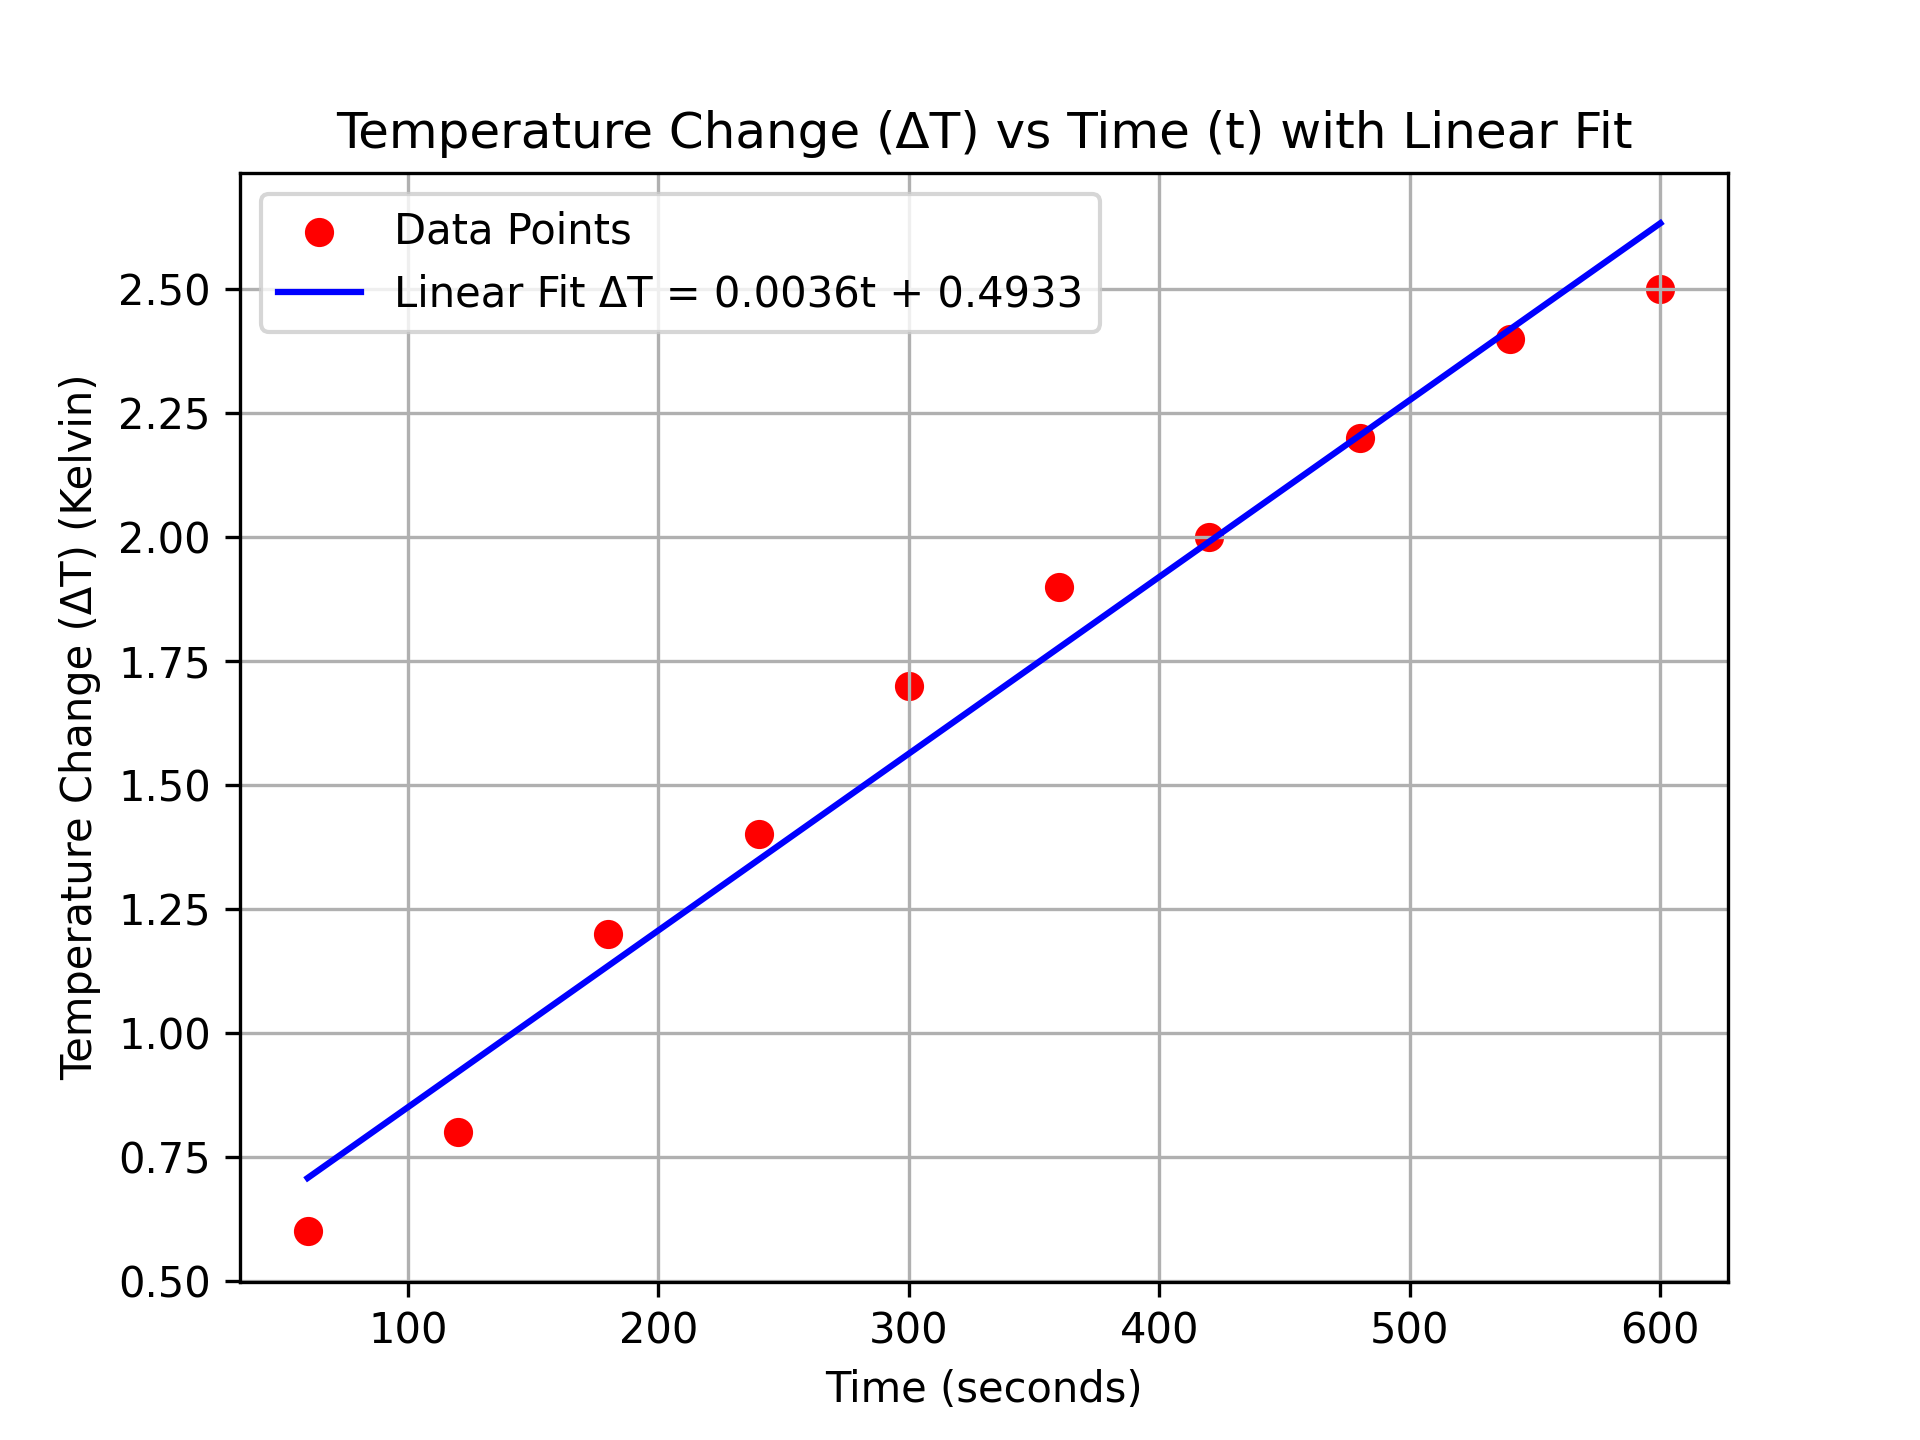
\includegraphics[width=0.95\linewidth]{../plots/DeltaT_vs_t_with_fit.png}
    \caption{Part II: $\Delta T(t)$ of the cold reservoir and its linear regression fit.}
    \label{fig:part2_deltat_fit}
\end{figure}

\begin{figure}[H]
    \centering
    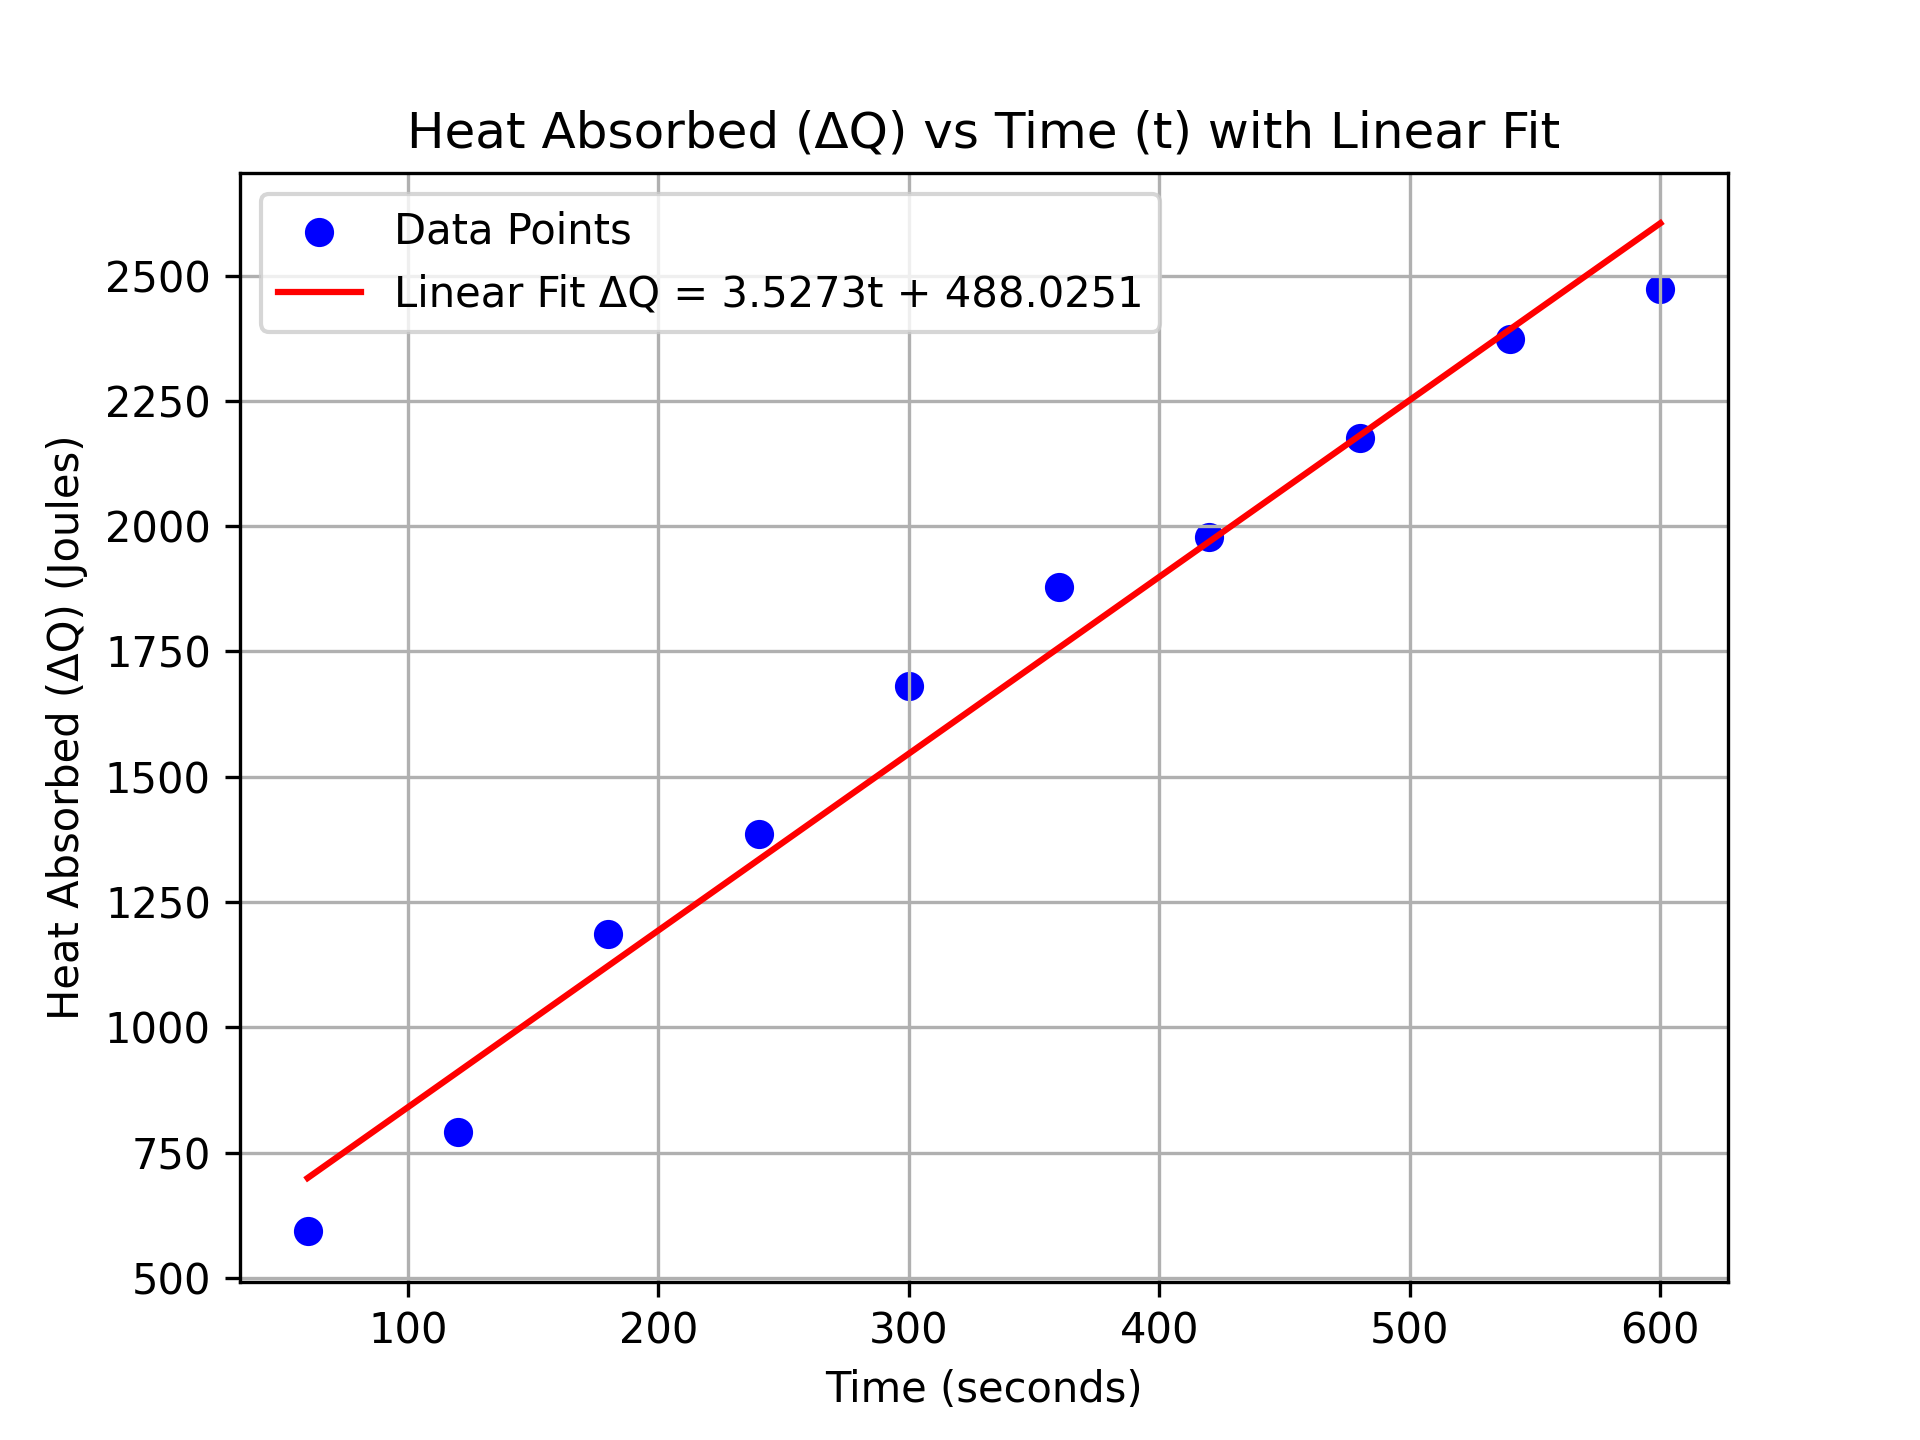
\includegraphics[width=0.95\linewidth]{../plots/DeltaQ_vs_t_with_fit.png}
    \caption{Part II: $\Delta Q_{\mathrm{env}}(t)$ and its linear regression fit.}
    \label{fig:part2_deltaq_fit}
\end{figure}

\begin{figure}[H]
    \centering
    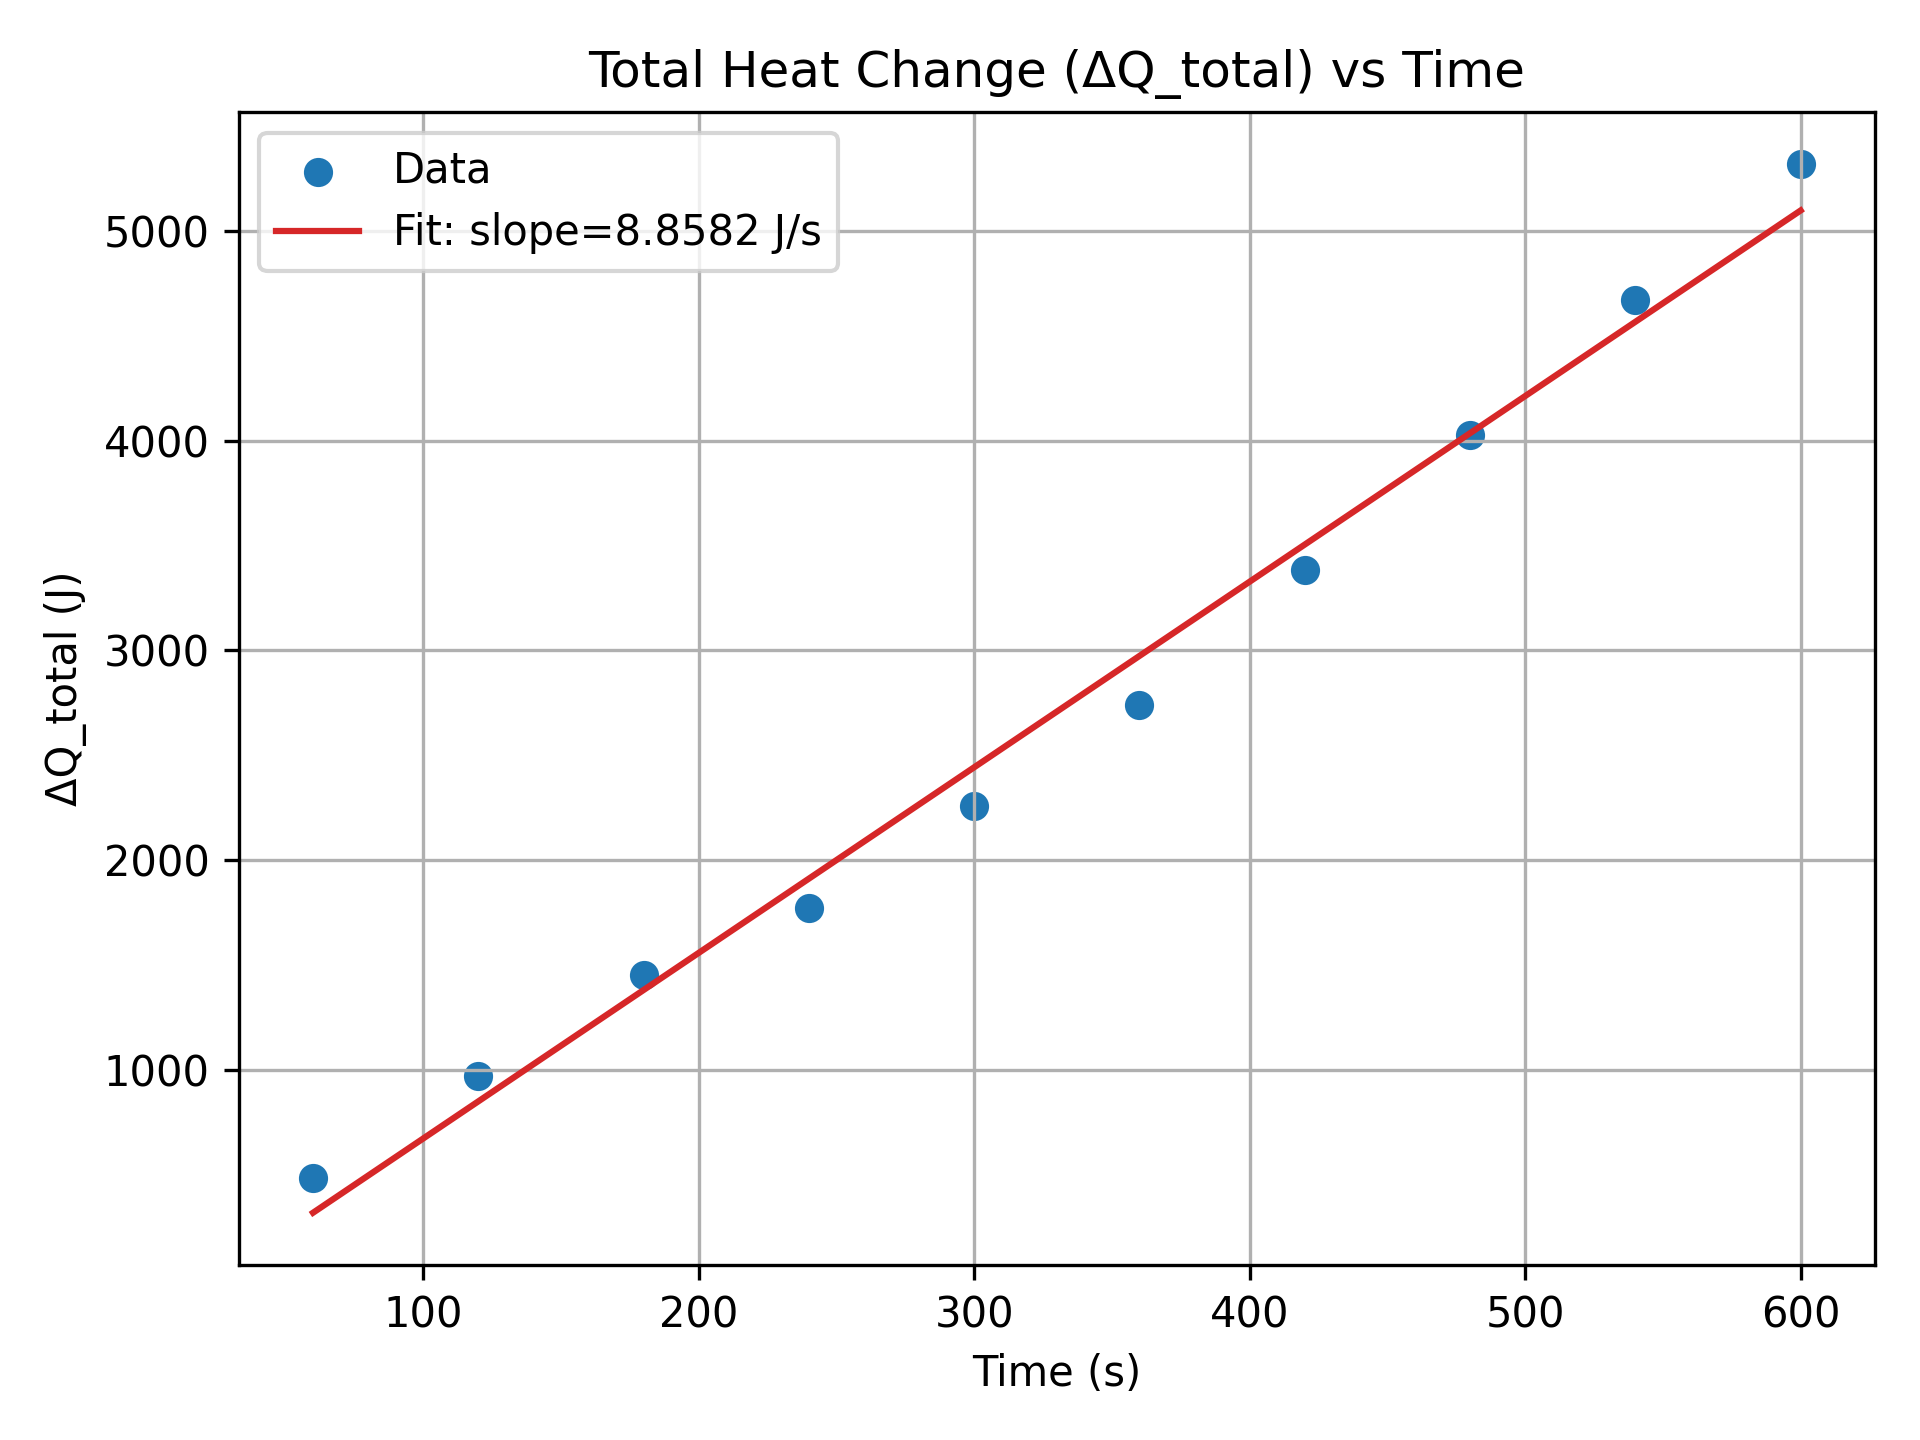
\includegraphics[width=0.95\linewidth]{../plots/DeltaQtotal_vs_t_with_fit.png}
    \caption{Part III: $\Delta Q_{\mathrm{total}}(t)$ and its linear regression fit used to estimate $dQ_{\mathrm{total}}/dt$.}
    \label{fig:part3_deltaqtotal_fit}
\end{figure}

\subsection{Processed Experimental Data}
To ensure reproducibility, the processed data tables were exported
as CSV files into \texttt{report/tables/}. Tables~\ref{tab:part2_processed} and
\ref{tab:part3_processed} are typeset directly from these exported CSV files.

\begin{table}[H]
\centering
\scriptsize
\caption{Part II processed table: $t$ in seconds, temperature, and computed $\Delta T$ and $\Delta Q_{\mathrm{env}}$.}
\label{tab:part2_processed}
\pgfplotstabletypeset[
    columns={t_s,T_K,DeltaT_K,DeltaQ_env_J},
    columns/t_s/.style={column name={$t$ (s)}},
    columns/T_K/.style={column name={$T$ (K)}},
    columns/DeltaT_K/.style={column name={$\Delta T$ (K)}},
    columns/DeltaQ_env_J/.style={column name={$\Delta Q_{\mathrm{env}}$ (J)}},
]{tables/part2_environment_processed.csv}
\end{table}

\begin{table}[H]
\centering
\scriptsize
\caption{Part III processed table: $t$ in seconds and computed $\Delta Q_{\mathrm{total}}$ along with the rod probe temperature difference.}
\label{tab:part3_processed}
\pgfplotstabletypeset[
    columns={t_s,T_K,DeltaT_K,DeltaQ_total_J,DeltaT_rod_K},
    columns/t_s/.style={column name={$t$ (s)}},
    columns/T_K/.style={column name={$T$ (K)}},
    columns/DeltaT_K/.style={column name={$\Delta T$ (K)}},
    columns/DeltaQ_total_J/.style={column name={$\Delta Q_{\mathrm{total}}$ (J)}},
    columns/DeltaT_rod_K/.style={column name={$\Delta T_{\mathrm{rod}}$ (K)}},
]{tables/part3_total_processed.csv}
\end{table}


% ---------- DISCUSSION ----------
\section{Discussion}
The regression-based determination of $dQ/dt$ provides a highly robust estimate of steady heat
flow because it utilizes the full time series rather than discrete point-to-point differences.
The high $R^2$ values for both the environmental ($R^2 \approx 0.978$) and total heat fits ($R^2 \approx 0.990$) 
mathematically validate the fundamental assumption of Fourier's law: the system had successfully 
reached a steady state ($\partial T/\partial t = 0$), resulting in a constant rate of heat transfer.

The computed calorimeter heat capacity ($2255.68\,\text{J/K}$) differs substantially from the manufacturer 
reference ($78\,\text{J/K}$). This extreme inflation is a known artifact of the open-air mixing procedure. 
During the transfer, significant heat from the hot water is lost to the ambient room air via convection 
and vaporization. Because the mathematical energy balance assumes an ideally isolated system, it incorrectly 
attributes all of this lost environmental heat to the calorimeter's thermal mass. Consequently, the 
manufacturer's established value of $78\,\text{J/K}$ was deemed physically realistic and was exclusively 
utilized for the subsequent thermal conductivity analysis.

Furthermore, the experimentally determined thermal conductivity of copper ($254.16\,\text{W}\,\text{m}^{-1}\,\text{K}^{-1}$) 
is lower than the widely accepted PHYWE literature value of $384\,\text{W}\,\text{m}^{-1}\,\text{K}^{-1}$. This 
deviation is expected for this specific macroscopic setup primarily due to radial heat loss; Fourier's law 
assumes strictly one-dimensional heat flow, but the uninsulated rod inherently radiates and convects thermal 
energy from its sides. Additionally, microscopic air gaps between the Pt100 surface probes and the rod can 
introduce thermal contact resistance, slightly suppressing the measured spatial temperature gradient.

Finally, regarding the electrical measurements, correcting the measured voltage for the instrumental amplifier 
gain of $10^4$ was physically critical. Without this scaling, the resistance would have been artificially 
inflated, resulting in a conductivity characteristic of a semiconductor rather than a highly conductive metal lattice.

% ---------- CONCLUSION ----------
\section{Conclusion}
The thermal and electrical conductivities of macroscopic metal rods were successfully determined using a 
reproducible, unit-consistent computational data pipeline. By utilizing continuous time-series linear regression 
to mathematically verify steady-state conditions and isolate the net heat flow, the thermal conductivity of copper 
was evaluated to be $\lambda_{\text{Cu}}=254.16\,\text{W}\,\text{m}^{-1}\,\text{K}^{-1}$. Additionally, by applying 
a 4-conductor Ohm's law measurement and rigorously correcting for the $10^4$ instrumental amplifier gain, the 
electrical conductivity of aluminium was accurately measured as $\sigma_{\text{Al}}=3.820\times10^{6}\,\Omega^{-1}\,\text{m}^{-1}$. 
These results demonstrate that accounting for parasitic environmental heat losses and absolute instrumental scaling 
is paramount for extracting physically realistic material constants in a laboratory setting.
% ---------- ADDITIONAL RESOURCES ----------
\section{Additional Resources}
Computational record: \url{https://github.com/ibeuler/LAB-Reports/blob/main/THERMODYNAMICS_AND_STATISTICAL_PHYSICS/4th_/Analysis/calculate.ipynb}.

\begin{figure}[H]
    \centering
    \begin{minipage}{0.15\textwidth}
        \centering
        \qrcode[height=1.5cm]{https://github.com/ibeuler/LAB-Reports}
    \end{minipage}%
    \begin{minipage}{0.2\textwidth}
        \raggedright
        \caption{Access the GitHub repository for source code and related experiments.}
        \label{fig:qr_code}
    \end{minipage}
\end{figure}

\begin{thebibliography}{9}
\bibitem{lab_manual}
    ISTANBUL UNIVERSITY, \textit{THERMODYNAMICS AND
STATISTICAL PHYSICS
LABORATORY LABORATORY EXPERIMENTS MANUAL}, Department of Physics.

% Add more references as needed

\end{thebibliography}

\end{document}